\documentclass{article}
\usepackage{xeCJK}
\usepackage{graphicx}
\linespread{1.1}
\setCJKmainfont{SimSun}
\title{LabReport on Extendible Hashing}
\author{10389048杨帆 \\ 10389084梁展瑞 \\ 12924901古宣佑}
\begin{document}
\maketitle
\begin{abstract}
    This is the LabReport about EHDB, a simple database system featured with the extendible hashing algorithm and the clock page replacement algorithm. In this report we provide some details about the ideas and implementation. Moreover, we will also discuss on the problems that trapped us and how we overcame them, and about the optimization of the EHDB. Thanks for Mr. Feng's and TAs's instructions.
\end{abstract}
\section{Environment}
    \begin{enumerate}
        \item Operating system: Linux(Debian \& Arch \& Ubuntu, with 3.0+ kernels)
        \item Language: C
        \item Compiler: GCC
        \item Documentation: \LaTeX , asciidoc, Markdown
        \item Collaboration Platform/Project Hosting: GitHub
        \item Debug utils: GDB, python, perf, gprof, xdot, gprof2dot, VIM(to do regex matching often)
        \item Editor: VIM
    \end{enumerate}
    \paragraph{}
        Here's the repo on GitHub, where you can see several branches, and some history about the project.
    \begin{verbatim}
        https://github.com/ddmbr/Extendible-Hashing/
    \end{verbatim}
\section{Overview}
    \paragraph{}
        What this program mainly do can be roughly divided into two aspects, namely \emph{build} and \emph{query}.
    \subsection{Build the database}
        \paragraph{}
            We have to parse the raw data before actually building the database. We then design our own data structure to store the data, which save a lot of space(will be discussed in the following sections).
        \paragraph{}
            When building the database, first of all the program extract records from the raw data, and translate them to the data structure we previously mentioned, formally called recotd\_t. 
        \paragraph{}
            Next, the key is extract from the record\_t, which decide its hash value and therefore the bucket it should be contained. The record\_t then go to the bucket it belongs to. Index and bucket are corresponding to the files \emph{index} and \emph{bucket}, and each 8K of the files represent a page of them.
        \paragraph{}
            When a bucket is full, it split and when necessary, the index is also doubled.
        \paragraph{}
            It is worth mentioning that, when the records in a bucket is impossible to distinguished only by their hash values, it make no sense to split the bucket. In this situation, a new bucket should be created to hold comming data, with a link pointing to the previous bucket.
        \paragraph{}
            Here's a draft\footnote{You can also see that on our GitHub Repo.} about the process.
\begin{verbatim}
While the end of the raw file(i.e, lineitem.tbl) is not reached, 
    Load a page from the raw file to the memory.
    Loop through the page, to:
        Read the next record in the page.
        Get its key.
        Get the hash value `hv' of the key.
        Fetch the corresponding index page,
        According to the index, fetch the corresponding
        bucket page.
        Before inserting the record, check that 
        whether the bucket will be overflowed.
            If yes,
                If global depth == local depth,
                    Double the index
            Then split the bucket and redistribute.
        Write the record into the page.

\end{verbatim}
    \subsubsection{Split Bucket}
        This is the most important part of the extendible hash algorithm. A bucket need to be splited when a new record is to be inserted into it but failed since the size limit. After the bucket spliting, the records in the old bucket are redistributed into two new buckets, and one of the new buckets will replace the old bucket. 

        The index need to be updated, too. Suppose a mapping \verb|(hv, oldBucketID)| exist before the spliting, then the mapping may change to either \verb|(hv, newBucketID)| or \verb|(hv, newBucketID2)|. We call the procedure remapping.

        When doing the remapping, we use a efficient method. Note that if two mapping \verb|(hv1, oldBucketID)| and \verb|(hv2, oldBucketID)| exist with the old bucket some localDepth, then the lowbits count to \verb|localDepth| bits of hv1 and hv2 are equal. So we don't need to scan all the index mapping and modify them. We need only scan the in \verb|{hv, hv + (1<<localDepth), hv + 2*(1<<localDepth), ...\}|. This improves the speed of the program by 10 times!
    \subsection{Query}
        \paragraph{}
            This process is much simply compared with the building process, with the folliwing steps:
\begin{verbatim}
While not reach the end of the query,
    Read next specific key.
    Get the hash value `hv' of the key.
    Fetch the corresponding bucket
    Loop through the bucket and print the matched records.
\end{verbatim}
\section{Architecture}
    \subsection{Main modules}
        \paragraph{}
            The program(we call it EHDB) consists of mainly 4 important modules, the File Manager, Buffer Manager, Parser and Hash.
        \begin{itemize}
            \item File Manager is responsible for the manipulation directly on the filesystem, for example request for a new page on disk.
            \item Buffer Manager deals with operations concerened with the main memory, like page swapping. It contains the core of the Clock Page Replacement Algorithm.
            \item Parser, as its name suggests, will parse raw data.
            \item Hash module contains the core of the Extendible Hashing algorithm.
        \end{itemize}
    \subsection{Organize the modules}
        \paragraph{}
            We experience some errors while trying to get the above modules well organized. Here we'd like to share our findings.
        \paragraph{}
            On the relationship among the Buffer manager, the Hash, and the Parser, we first designed it like this:
        \paragraph{} 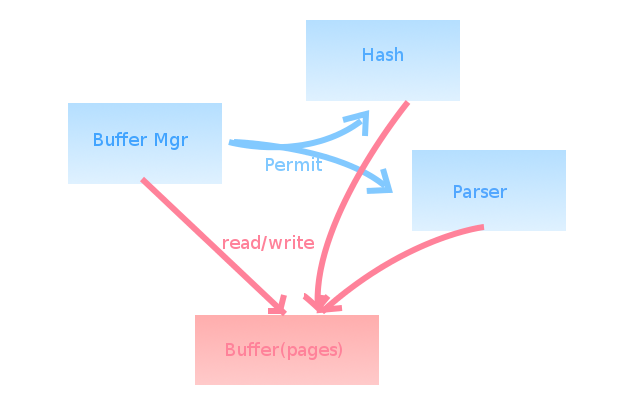
\includegraphics[scale=0.5]{img/arch1.png}
        \paragraph{}
            Notice that in this diagram we omit the File Mgr and some smaller module, as they are no concerned with the problem that we will then talk about.
        \paragraph{}
            According to this idea, the Buffer Manager is responsive for giving permission to the Parer and the Hash module. After aquiring its permission, the two modules then manipulate the data in the buffer directly. However it's hard to guarentee that while the 3 modules can deal with the data directly(by aquiring its memory address), they can also do it in a orderly manner. Therefore data inconsist \emph{will} occur, which turn out to be a disaster.
        \paragraph{}
            This problem, however, can be fixed by assigning the \emph{hold} flag to each page of data, prevent it from being modified by 2 or more modules. But all the modules and their methods, should then be able to set and reset the flag correcty, hence add to the complexity of programming.
        \paragraph{}
            We finally came up with a more convenient solution.
        \paragraph{} 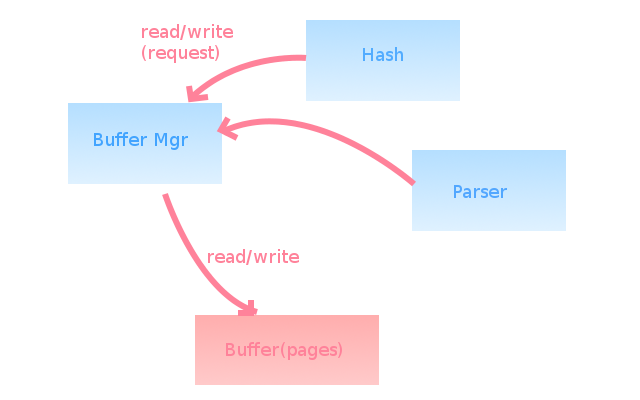
\includegraphics[scale=0.5]{img/arch2.png}
        \paragraph{}
            A layer was construted upon the Buffer Manager, forcing all requests to go through it. Although this slows down the program a bit, it effectively prevents potential access violations. This strategy works well and turns out to be a reliable one.
    \subsection{Algorithms}
        \begin{enumerate}
            \item Clock Page Replacement Algorithm
                \paragraph{}
                    Clock Page Replacement Algorithm is a more efficient version of FIFO. The clock algorithm keeps a circular list of pages in memory, with the "hand" (iterator) pointing to the last examined page frame in the list. When a page fault occurs and no empty frames exist, then the R (referenced) bit is inspected at the hand's location. If R is 0, the new page is put in place of the page the "hand" points to, otherwise the R bit is cleared. Then, the clock hand is incremented and the process is repeated until a page is replaced.
                \paragraph{}
                    In another word, the replacement(or swaping) works just as follows
                    \begin{enumerate}
                        \item If the R bit of the page pointed by the head equals to 0, swap that page.
                        \item Otherwise, set the R bit to 0, and the hand then point to the next page in the clock.
                        \item Repeat until the a page with R=0 is found.
                    \end{enumerate}
                \paragraph{}
                    R is set 1 for the new page swapped in.
            \item Extendible Hashing
                \paragraph{}
                    Extendible Hashing is a type of hashing system which treats a hash as a bit string. Because of the hierarchical nature of the system, re-hashing is an incremental operation (done one bucket at a time, as needed). This means that time-sensitive applications are less affected by table growth than by standard full-table rehashes.
                \paragraph{}
                    There're 2 version of this algorithm, the LSB version and the MSB one. There exits some differences and will do analysis on this in the later section.
        \end{enumerate}
    \subsection{Data structures}
        \subsubsection{Record}
            \paragraph{}
                Here's the record\_t structure in our codes.
\begin{verbatim}
struct record_t{
    identifier_t orderkey, 
               partkey, 
               suppkey;
    int linenumber;
    decimal_t quantity,
            extendedprice,
            discount,
            tax;
    flag_t returnflag,
           linestatus;
    date_t shipdate,
           commitdate,
           receiptdate;

    char shipinstruct[25+1];
    char shipmode[10+1];
    char comment[44+1];
};
\end{verbatim}
            \paragraph{}
                in ehdb\_record.h, we provide some methods about the records. The two most important functions may be these two
\begin{verbatim}
/* read and convert a record from `page` start with `offset`
 * return: the new offset when conversion finished
 *
 * Example usage:
 *
 * int offset = 0
 * page_t * page = ...;
 * record_t record;
 * while(offset != -1){
 *      offset = ehdb_page_record2record(page, offset, &record);
 *      // do something or print out the record
 *      //...
 * }
 */
int 
ehdb_page_record2record(page_t * page, int offset, record_t * record);

/* convert record_t and write it back
 * to a page on disk
 */
void 
ehdb_record2page_record(record_t * record, int bucket_id);
\end{verbatim}
        \subsubsection{Page}
            \paragraph{}
                Here's the page\_t structure in our codes.
\begin{verbatim}
struct page_t{
    page_type_t page_type;
    int page_id;
    void * head;
    short modified;
};
\end{verbatim}
            \paragraph{}
                We use a flag called \emph{modified}, to record that whether the page has been modified since fetched from the disk. Then Buffer Mgr will then be able determine whether a ``save'' operation is necessary, which is an improvement on I/O effeciency.
\section{Analysis and Optimization}
    \subsection{Compare the LSB and MSB strategy}
        \paragraph{}
            To help us comphrehense the idea of extendible hashing better, and ease the debugging, we rerwrite the program in Python(\verb|hash.py,hhash.py| in the src folder), which is both shorter and more comphrehensive(about 250 lines and it can show the process of hashing). Then we generated an animation and got a feel about how the bucket split and how the index double.
        \paragraph{} 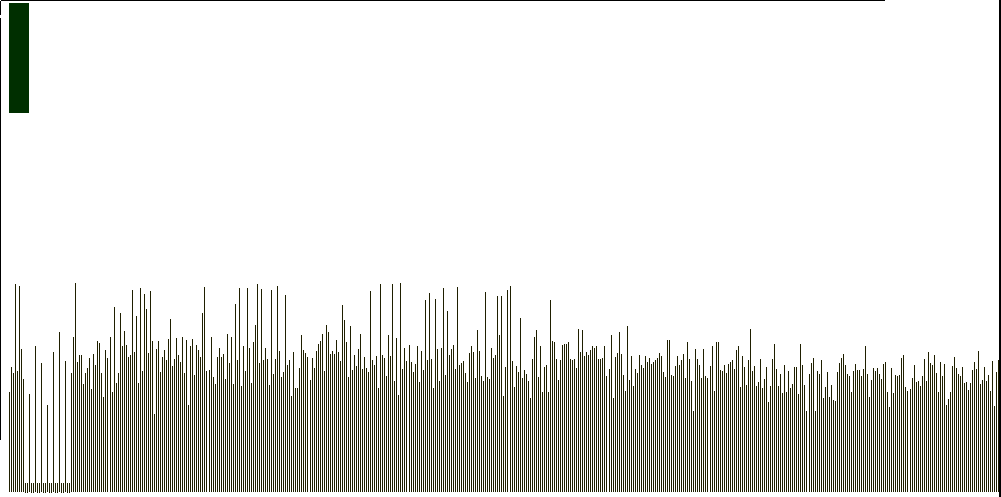
\includegraphics[scale=0.4]{img/pic20000_l.png}
        \paragraph{}
            The graph above describes the pages of index(4 pages) and buckets(Many!), with the LSB hashing strategy and 20000 raw records. With some observation we confirmed that the usage rate of a bucket is about 70\%. 
        \paragraph{} 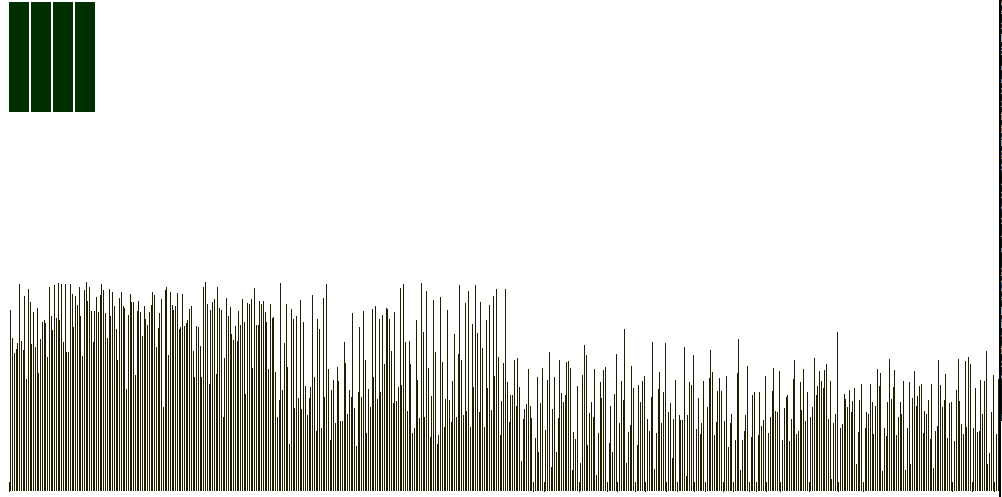
\includegraphics[scale=0.4]{img/pic20000_h.png}
        \paragraph{}
            Then the MSB strategy. We see that the MSB strategy consume more storage and with lower usage rate of bucket. Howver it's much faster. Here's a list about the different version and the corresponding IO frequency.
        \begin{itemize}
            \item 8 pages buffer, LSB, 107857 IOs
            \item 8 pages buffer,MSB, 67844 IOs
            \item 128 pages buffer, MSB,12227 IOs
            \item 128 pages buffer, LSB,99591 IOs
        \end{itemize}
        \paragraph{}
            Larger buffer definetely helps improve IO performance. However there's a flaw about it, which we will discuss later.
    \subsection{The record structure}
        \paragraph{}
            To help optimize the program, we generate a profile diagram\footnote{More diagrams can be found in doc/img/} about it.
        \paragraph{} 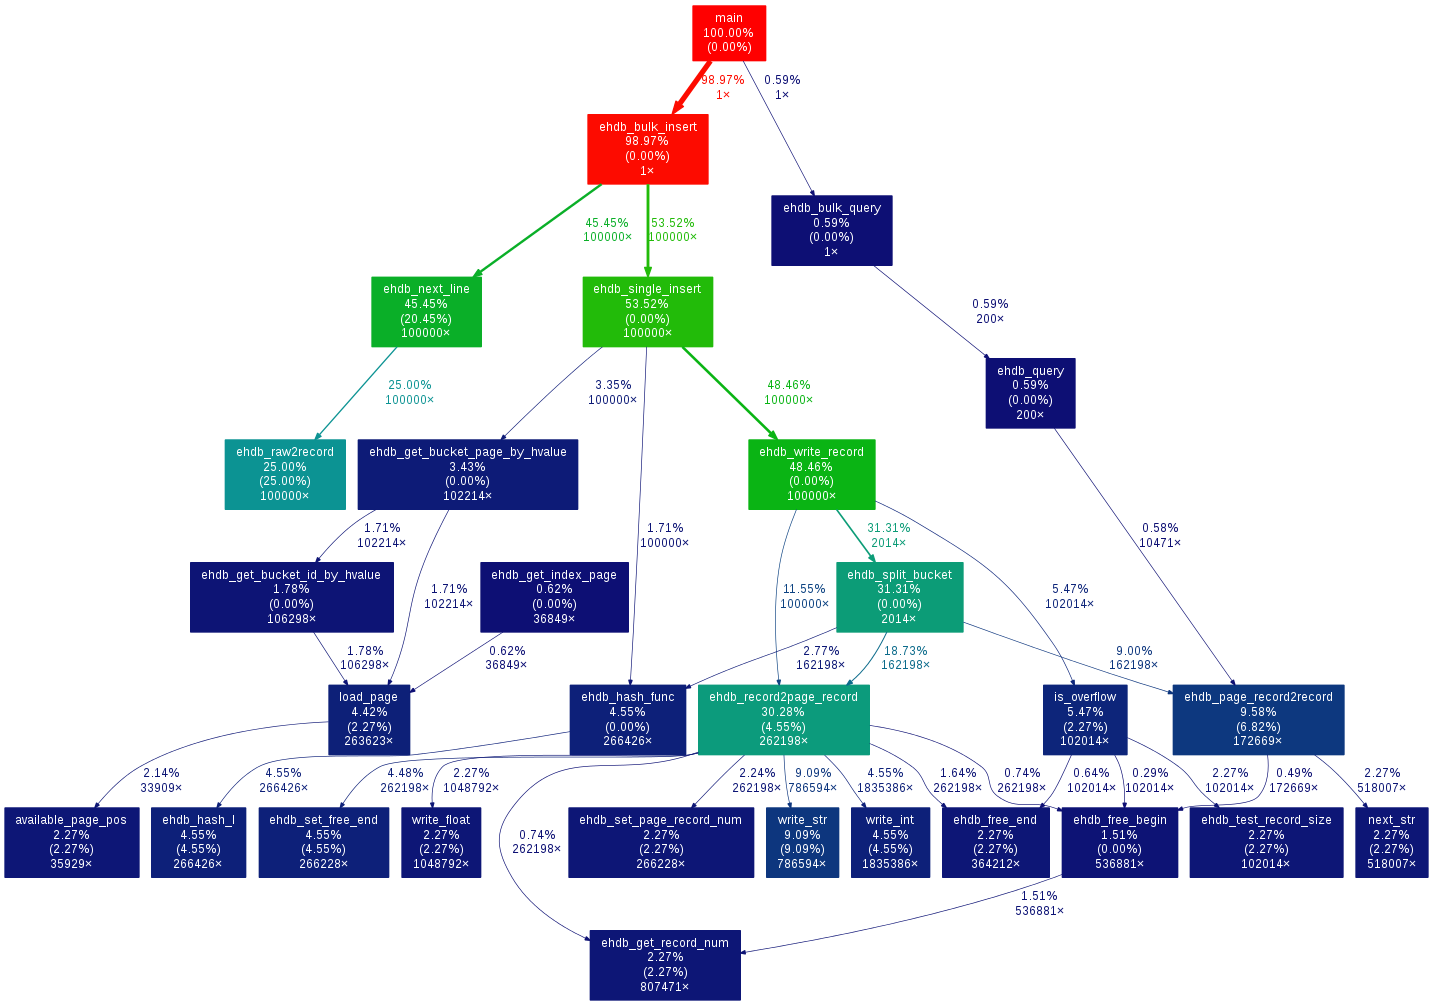
\includegraphics[scale=0.3]{img/proff_big_record.png}
        \paragraph{}
            It says that the translate(raw data<->record<->page record or say disk files) of records cost a lot of CPU time.\footnote{In the previous discussion we stated that a special data structure is designed to hold a single record, it can save disk space} However it is not surprising because we use sscanf to convert. To do some comparations, we then rewrite a new version of EHDB, which doesn't do the translation. Records are stored simply as a char string in this version.
        \paragraph{}
            It turned out that, the new version is slower, by about 2min. Based on these facts, we can conclude that the trade-off between IO time and CPU time we previously took is \emph{worthwhile}.
    \subsection{Cache}
        \paragraph{}
            As buffer grows bigger, it takes more time for Buffer Mgr to search for a specific page in the buffer. Then we came up with an idea. We design a cache algorithm, which stores 2 recently used pages' ID. When the user program require a page, the buffer manager will scan the cache for the required page. After the test we made, we found that the cache hit rate\footnote{(cache hit count)/(buffer hit count)} of the LSB hash is about 75\%, while in MSB 95\%. We can believe that in most time the cache is helpful. 
        \paragraph{}
            We compare the 128 pages buffer with cache and the one without cache, and discover that the cache is indeed a great help. It decrease the total time cost by about 10\%.
    \subsection{More optimization}
        \paragraph{}
            We have more thoughts on this project, however time is limit. Here are two other ideas that we are interested in.
        \begin{itemize}
            \item How about adjust the page size? Once in MSDN, I see that the Microsoft staff have test various page size, from 4K, 8K, to even 64K(should be 4*n K as most filesystem transfer 4K data a time). And they discover that 8K is the best choice. We are interested in doing it by ourselves and exploring the reason.
            \item We think the clock algorithm is not so effective. A buffer manager based on Red-Black tree\footnote{The famouse CFS strategy in Linux Kernel code is based on Red-Black tree data structure.} or Splay tree might have more advantage. It's a kind of trade-off. With more complex algorithm, we use CPU time to trade the I/O time.
        \end{itemize}
\section{Summary}
    \paragraph{}
        We learn a lot, and have a lot of fun from this project. The most important thing is that, we are strongly impressed by the characteristics of the C programming language. It is not so human-friendly like Python, but it can be used to control the data and process in a very effective way(I mean the program's effeciency, not the development). However it also troubles us a lot and we admit that we aren't familiar with its feature much.
    \paragraph{}
        And this project also gives us a more detailed view, about how a DBMS actually works.
\end{document}
